\documentclass{article}
\usepackage{arxiv}

%\usepackage[utf8]{inputenc} % allow utf-8 input
\usepackage[T1]{fontenc}    % use 8-bit T1 fonts
\usepackage{hyperref}       % hyperlinks
\usepackage{url}            % simple URL typesetting
\usepackage{booktabs}       % professional-quality tables
\usepackage{amsfonts}       % blackboard math symbols
\usepackage{nicefrac}       % compact symbols for 1/2, etc.
\usepackage{microtype}      % microtypography
\usepackage{indentfirst}
%\usepackage{lipsum}		% Can be removed after putting your text content
\usepackage{graphicx}
\usepackage{natbib}
\usepackage{doi}
\usepackage{array}
\usepackage{algorithm}  
\usepackage{algorithmic}
\usepackage{subfigure}
\renewcommand{\algorithmicrequire}{\textbf{Input:}} % Use Input in the format of Algorithm
\renewcommand{\algorithmicensure}{\textbf{Output:}} % Use Output in the format of Algorithm

\setlength{\parindent}{1em}

\title{Mid-air Collision Avoidance Based on Deep Distributed Multi-Agent Reinforcement Learning}

%\date{September 9, 1985}	% Here you can change the date presented in the paper title
%\date{} 					% Or removing it

\author{ \href{https://orcid.org/0000-0001-7508-7567}{
\includegraphics[scale=0.06]{orcid.pdf}\hspace{1mm}Weilin Cai}\\
%\thanks{Use footnote for providing further
%		information about author (webpage, alternative
%		address)---\emph{not} for acknowledging funding agencies.} \\
	School of Science and Engineering\\
	The Chinese University of Hong Kong\\
	Shenzhen, Guangdong 518172 \\
	\texttt{weilincai@link.cuhk.edu.cn} \\
	%% examples of more authors
	\And
	\href{https://orcid.org/0000-0001-9936-4899}{
\includegraphics[scale=0.06]{orcid.pdf}\hspace{1mm}Chi Li} \\
	School of Science and Engineering\\
	The Chinese University of Hong Kong\\
	Shenzhen, Guangdong 518172 \\
	\texttt{chili@link.cuhk.edu.cn} \\
	%% \AND
	%% Coauthor \\
	%% Affiliation \\
	%% Address \\
	%% \texttt{email} \\
	%% \And
	%% Coauthor \\
	%% Affiliation \\
	%% Address \\
	%% \texttt{email} \\
	%% \And
	%% Coauthor \\
	%% Affiliation \\
	%% Address \\
	%% \texttt{email} \\
}

% Uncomment to remove the date
%\date{}

% Uncomment to override  the `A preprint' in the header
\renewcommand{\headeright}{Final Project Report}
\renewcommand{\undertitle}{Final Project of DDA6105/CIE6023 Reinforcement Learning}
\renewcommand{\shorttitle}{MACA Based on D2MARL}

%%% Add PDF metadata to help others organize their library
%%% Once the PDF is generated, you can check the metadata with
%%% $ pdfinfo template.pdf
\hypersetup{
pdftitle={A template for the arxiv style},
pdfsubject={q-bio.NC, q-bio.QM},
pdfauthor={David S.~Hippocampus, Elias D.~Striatum},
pdfkeywords={First keyword, Second keyword, More},
}

\begin{document}
\maketitle

\begin{abstract}
	A mid-air collision is an accident where two aircraft come into contact with each other while both are in flight, which could result in a disaster. To avoid such casualties, effective air traffic control, which is generally recognized as a real-time and safety-critical decision-making process in periodic flight phases, becomes a necessity. With the fast-growing air traffic density and complexity in traditional controlled airspace, an autonomous air traffic system is needed as the ultimate tool to accommodate and handle stochastic, dense and dynamic operational scenarios, and to provide tactical and practical strategies for air traffic controllers. In our work, we avoid mid-air collision by control the velocity, considering both the speed and the direction, to maintain safe separation. We propose a deep multi-agent reinforcement learning framework to perform aircraft conflicts detection and resolution in designated en-route sector with multiple intersections and emerging points. Our proposed framework applies a policy-based learning method, Proximal Policy Optimization (PPO) to help stabilize the converged process. We plan to use the BlueSky application as the simulation environment to train and evaluate our model.
\end{abstract}


% keywords can be removed
\keywords{Mid-air collision avoidance \and Air traffic control \and Multi-agent reinforcement learning}

\section{Introduction}
In the past 50 years, we've seen many severe aviation accidents, while among which the collision of two aircraft in the air is considered the most appalling ones, as they caused the worst of the losses for both sides of the collision. According to European Union Aviation Safety Agency (EASA), such accidents can be defined as mid-air collision \citep{de2011use}. To avoid mid-air collision, the concepts of air traffic confict and safety zone are set by specialized agencies. In China, two aircraft are considered in-conflict if they had a distance less than 5 nautical miles horizontally and 300 meters vertically, and such space that keep safety separation is defined as the safety zone. With these concepts introduced, there are actually more cases of air traffic conflict than mid-air collision although the planes did not collide. To avoid mid-air collision, currently people rely on air traffic control (ATC) to reduce air traffic confict. With the fast growth of global air traffic density and complexity, it becomes a big challenge to ensure effective ATC. However, nowadays tatical decisions are still being made by human air traffic controllers, with the mechanism of which remains largely the same as that of 50 years ago \citep{national2014autonomy}.

The density could increase a lot when it comes to low-altitude airspace traffic, while the behaviors of aircraft become more complex \citep{kopardekar2015safely}. What's more, the vertical separation distance is harder to maintain and one airway can no longer contain as many flight levels as that in high-altitude airspace due to the limited ground clearance. One solution is to strictly divide aircraft activities into disjoint space, but this could cause low throughput which really matters at high traffic density. Therefore, some strategy like time-division multiplexing, which allows the aircraft to pass the same space at different time is inevitably adopted \citep{mueller2017enabling}. In such cases, we need real-time autonomous ATC systems to decide the aircraft actions, most possibly to change the velocity, to avoid potential mid-air collision in some specific sector.

For real-time autonomous ATC within high-density airspace, traditional optimizing methods might not be ideal solutions. To get optimal solution under such conditions, traditional approaches require global information of all aircraft in the sector and made centralized decisions\citep{farley2007fast}. Note that such process is rather time-consuming, and it also takes time for aircraft to make reactions to the orders given by a central controller like the airport traffic control tower. Considering that the process is latency-sensitive, the approach of reinforcement learning could be a better choice. Although it's slow to train a reinforcement learning model, it's very quick for the model to make interpretation \citep{brittain2019autonomous}. Therefore, it's applicable for each aircraft to use reinforcement learning methods to make instant decision. What's more, as long as the model is pretrained before loaded into each aircraft, the procedure of making en-route advisories will not cause unacceptable computational pressure.

The structure of the paper is organized as follows. Section 2 reviews the background and  related work. In Section 3, our detailed models, proposed algorithm and environment settings will be introduced. Section 4 presents our experiment results via our designed framework, followed by conclusions and future works in Section 5. Lastly, in the appendix, we briefly introduce the schedule and contribution, and the repository of our project on \emph{Github}.
\section{Background}

In the past few decades, many great research contributions and effective decision tools have been implemented to the topic of collision avoidance in air traffic control. Autoresolver, a well-known physics model-based approach, can efficiently generate a series of conflict-free trajectories by employing an iterative method to satisfy all conflict resolution conditions \citep{farley2007fast}. In response to our research focus, the specified sector with multiple intersections and emerging points, National Aeronautics and Space Administration (NASA) has introduced a centralized scheme, known as Traffic Mangement Advisor (TMA) to design such no-conflict time slots and then make sure to maintain seperation distance \citep{erzberger2014design}. In recent years, Artificial intelligence (AI)    technology has been widely used in air traffic management, especially under uncertain decision-making environments which requires highly precise and fast-time simulators to make interaction with the agent. In this way, we employed Bluesky \citep{hoekstra2016bluesky} as our validation framework which was designed by TU Delft and has been extensively applied to relistic and real-time air traffic scenarios.

Multi-agent techniques has seen great success in solving issues related with conflict seolutions and collision avoidance. In early study \citep{wollkind2004automated}, an aircraft was regarded as an agent and negotiation skills were emphasized to resolve appeared conflict warnings. However, in recent works, such communication techniques aren't generally imposed and naturally agents are free to learn the ability through continuous training \citep{brittain2020deep}. Besides, some decentralized algorithms such as multi-agent Monte Carlo Tree Search (MCTS) \citep{yang2020scalable} and Markov Decision Process (MDP) \citep{bertram2020distributed} are formulated to predefine loss of separation (LOS). The LOS situation is introduced from aircraft safety spearation, as shown in Figure \ref{fig:los}. Due to the characteristcs of decentralized framework, these algorithms present priorer performance and faster convergence rate to those with the centralized scheme.

\begin{figure}[H]
    \centering
    \subfigure[Aircraft Safety Separation]{
        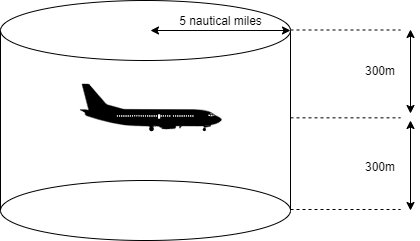
\includegraphics[width=0.365\columnwidth]{images/space.png}
    }
    % \subfigure[$(\epsilon=0.6, T=750)$]{
    %     \includegraphics[width=0.46\columnwidth]{pic/convergence_4-16_n10_ep0.6_T750.png}
    % }
    \subfigure[An Example of LOS]{
        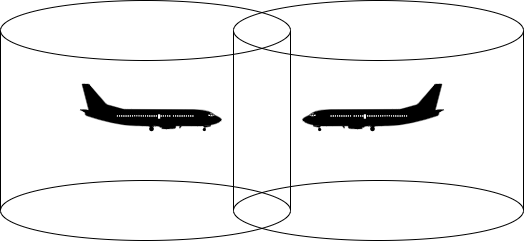
\includegraphics[width=0.46\columnwidth]{images/los.png}
    }
    \caption{The Concept of Aircraft Safety Separation and Loss of Separation}
    \label{fig:los}
\end{figure}

The worst and serious case of LOS could be mid-air collision, and at low altitude, cross-level actions to avoid collision is not commonly applicable, as shown in Figure \ref{fig:collision_level_change}. AI agents such as Alpha Go have shown tremendous advantages in imitating and learning sophisticated human behaviors and even defeated human in some highly dynamic and uncertain competition games through reinforcement learning \citep{mnih2015human}. First related work in aircraft collision avoidance can be traced to \citep{brittain2018autonomous}, where conflicts and delay mitigation are simultaneously emphasized. Then, \cite{pham2019machine} introduces randomness and scenarios analysis to the formulation of the aircraft' maneuvor. However, these approaches fail to consider speed as a vector and the sector structure with multiple emerging points. With this regard, we dedicated to further improve the existing implementation by considering more complex and practical scenarios.

\begin{figure}[H]
    \centering
    \subfigure[Aircraft Safety Separation]{
        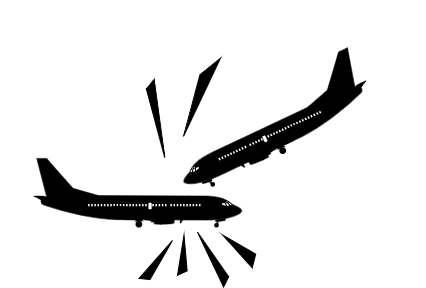
\includegraphics[width=0.35\columnwidth]{images/Mid-air_Collision.png}
    }
    % \subfigure[$(\epsilon=0.6, T=750)$]{
    %     \includegraphics[width=0.46\columnwidth]{pic/convergence_4-16_n10_ep0.6_T750.png}
    % }
    \subfigure[An Example of LOS]{
        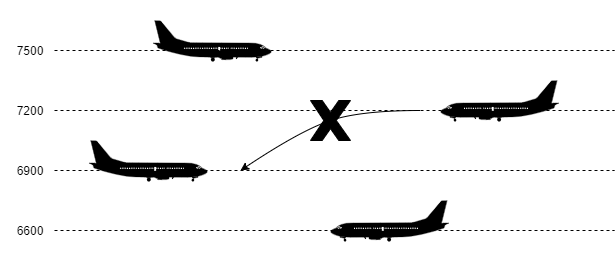
\includegraphics[width=0.46\columnwidth]{images/change_height.png}
    }
    \caption{Mid-air Collision and Flight Level Change Constraint}
    \label{fig:collision_level_change}
\end{figure}

In this work, a distributed deep multi-agent reinforcement learning framework (D2MARL) is proposed to tackle mid-air collision avoidance problems in the sector with multiple intersections and emerging points. 
\section{Approach}
In this section, we discuss the detailed process of problem formulation, including the relevant model objective and assumptions, and the definition of elements in our proposed multi-agent reinforcement learning model for collision avoidance. Besides, we present our proposed algorithm framework and related environment settings in our simulation experiments.

\subsection{Modeling}
The objective in our case studies is to ensure sufficient safe separation and avoid collision between aircrafts by providing speed advisories. The agents needs to learn and coordinate to maintain safe separation at every time step under stochastic and dynamic environment. Since our experiments are implemented on the Bluesky simulator, performance metrics assumptions related to different aircraft type and flight rules are predefined. Here we indroduce thorough formulation of the D2MARL problem by representing each aircraft as an agent and defining the corresponding state space, action space, termniation criteria and reward function.

\subsubsection{State Space}
The state information for the ownship contains the distance to the target, speed, speed change, direction variation, route identifier and the loss of separation distance. For the intruders, except the corresponding information for the ownship, their state space also concludes the mutual distance among ownship, intersection and the intruder self. An intersection plays a important part in defining a potential conflict between the ownship and intruders. Thus, we make the following assumptions that aircraft, which is either on the same route or in the conflicting route, must not have reached the intersection on conflicting route. 

Specifically, the state information for the ownership and the intruder are given respectively as follows:


$$s_t^o = \left( {d_{{\rm{goal}}}^{(o)},{v^{(o)}},{a^{(o)}},{d_l^{(o)}},{r^{(o)}},LOS} \right)$$

$$h_t^o\left( i \right) = \left( {d_{{\rm{goal}}}^{(i)},{v^{(i)}},{a^{(i)}},{d_l^{(i)}},{r^{(i)}},d_o^{(i)},d_{{\mathop{\rm int}} }^{(o)},d_{{\mathop{\rm int}} }^{(i)}} \right)$$

As listed above, the state at time $t$ consists of two part, the ownship state $s_t^o$ and the state of intruders $h_t^o$ that is available to the ownship. Here we explain the symbols in the state. Note that we don't put ownership's distance to the intersection into the ownership state, since one aircraft might encounter more than one intersection, and the dimension of the state can not be fixed then. Therefore, we can put such information into the intruders' state so that every intruder will have one and only one term of $d_{int}^{(o)}$ will be added, while $d_{int}^{(o)}$ is for the \textit{i-th} intruder's distance to the intersection. $d_{goal}^{(o)}$ and $d_{goal}^{(i)}$ descrbie the ownership's and the \textit{i-th} intruder's distance to the its goal. Similarly, to discribe other state information of the ownership and the \textit{i-th} intruder, we use $v$ for the velocity, $a$ for the last action taken, $d_l$ for the distance away from the airline, and $r$ for the airplane's radius which is useful for checking collisions. The $LOS$ value could varies depending on the aircraft type, but here we keep it the same just as supplementary information. $d_o^{(i)}$ describes the distance between the ownership and the \textit{i-th} intruder. Figure \ref{fig:intersect} and Figure \ref{fig:airway} explain the setting of the state space.

\subsubsection{Action Space}
The action space here could change according to our experiment settings. An action could be described as "to change the speed" or "to change the direction". To make the action space more complex, it could be described as "to change both of them", that is, "to change the velocity". More details are shown in Section \ref{sec:experiment}, the experiment part.

\subsubsection{Terminal State}
In each episode, a certain number of aircraft will be generated and the current state will come to an end if the following conditions are satisfied:

\[{N_{aircraft}} = 0\]

\subsubsection{Reward Function}
For any agent, the rewrad funtion are the same but the cooperation between the agents are encouraged. More precisely, if two agents are in a collision, they will receive a penalty. We define confict as the distance between two agents is less than 3 nautical miles, that is ${d^{LOS}} = 3$. Besides, the reward function is designed for the agents:

\[{r_t} = \left\{ {\begin{array}{*{20}{l}}
    { - 1}&{\rm{ if } \ d_o^c < 3 \ \rm{ or } \ |d^{(o)}_l| > r_a }\\
    { - \alpha  + \beta  \cdot d_o^c}&{\rm{ if } \ d_o^c < 10 \ \rm{ and } \ d_o^c \ge 3}\\
    0&{{\rm{ otherwise }}}
    \end{array}} \right.\]

Where $d_o^c$ is the distance between the ownship and the closest aircraft in nautical miles. $\alpha $ and $\beta $ are the penalty parameters for losing safe separation. By definition, the agents will learn to choose suitable action to maintain the distance requirements. If the $d_o^c < 3$ is violated, it indicates the loss of separation. Note that $d_l^{(o)}$ refers to the distance from the ownership plane to the airline, and $r_a$ refers to the maximum distance that is allowed to be away from the airline. The $|d^{(o)}_l| > r_a$ inequation is considered when direction changes are allowed in the action space. Figure \ref{fig:action} describes the settings for possible actions.

\begin{figure}[!htbp]
    \centering
    \subfigure[\label{fig:intersect}Intersection in a Sector]{
        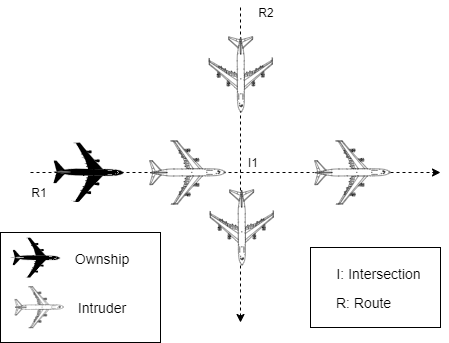
\includegraphics[width=0.3\columnwidth]{images/intersect.png}
    }
    \subfigure[\label{fig:airway}Airline and Airway]{
        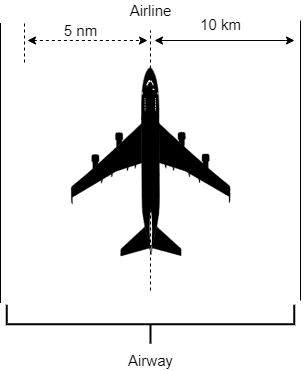
\includegraphics[width=0.18\columnwidth]{images/airway.png}
    }
    \subfigure[\label{fig:action}Possible Actions]{
        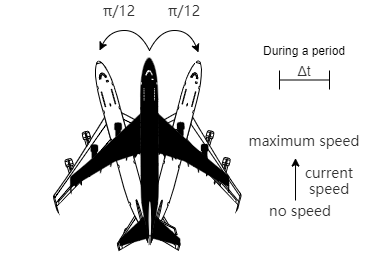
\includegraphics[width=0.3\columnwidth]{images/action.png}
    }
    \caption{State and Action Settings}
    \label{fig:state_action}
\end{figure}


\subsection{Algorithm}
Reinforcement learning can be briefly divided into model-based and model-free methodologies while model-free reinforcement learning can be further classified into value-based and policy-based algorithm. Considering the dynamics in state transition of aircraft movements is hard to determine, and policy-based algorithm is capable to learn stochastic policies where policy gradient direction can increase the possibility of better-than-average actions, we choose Proximal Policy Optimization (PPO) \citep{schulman2017proximal}, a recent policy-based algorithm that uses a neural network to approximate both the policy and the value function, as our basic algorithm framework. The alogorithm process is constructed as below: 
\begin{algorithm}[H]
    \caption{PPO-Clip}
    \begin{algorithmic}[1]
        \REQUIRE
        initial policy parameters $\theta_{0}$, initial value function parameters $\phi_{0}$
        
        \textbf{for} $k=0,1,2, \ldots$ do
        
        1. Collect set of trajectories $\mathcal{D}_{k}=\left\{\tau_{i}\right\}$ by running policy $\pi_{k}=\pi\left(\theta_{k}\right)$ in the environment.

        2. Compute rewards-to-go $\hat{R}_{t}$

        3. Compute advantage estimates, $\hat{A}_{t}$ based on the current value function $V_{\phi_{k}}$.

        4. Update the policy by maximizing the PPO-Clip objective via stochastic gradient ascent with Adam:
$$
\theta_{k+1}=\arg \max _{\theta} \frac{1}{\left|\mathcal{D}_{k}\right| T} \sum_{\tau \in \mathcal{D}_{k}} \sum_{t=0}^{T} \min \left(\frac{\pi_{\theta}\left(a_{t} \mid s_{t}\right)}{\pi_{\theta_{k}}\left(a_{t} \mid s_{t}\right)} A^{\pi_{\theta_{k}}}\left(s_{t}, a_{t}\right), \quad g\left(\epsilon, A^{\pi_{\theta_{k}}}\left(s_{t}, a_{t}\right)\right)\right)
$$

5. Fit value function by regression on mean-squared error via gradient descent algorithm:
$$
\phi_{k+1}=\arg \min _{\phi} \frac{1}{\left|\mathcal{D}_{k}\right| T} \sum_{\tau \in \mathcal{D}_{k}} \sum_{t=0}^{T}\left(V_{\phi}\left(s_{t}\right)-\hat{R}_{t}\right)^{2}
$$

\textbf{end for}   
    \end{algorithmic}
\end{algorithm}
We also consider multi-agent reinforcement learning, where a set of agents share the same environment, as presented in \ref{fig:multi_agent}.The difficulty for an agent lie in how to tackle the relationship between the environments and other agents to obtain a higher reward. In our paper, a centralized learning and decentralized execution framework is introduced. In this way, agents can be trained simultaneously by applying a centralized method where communication is encouraged to implement. It shows that centralized learning can improve the agents' learning efficency while decentralized schemes have an advantage under partial observability and in limited communications during execution \citep{foerster2017counterfactual}.

\begin{figure*}[htbp]
    \centering
    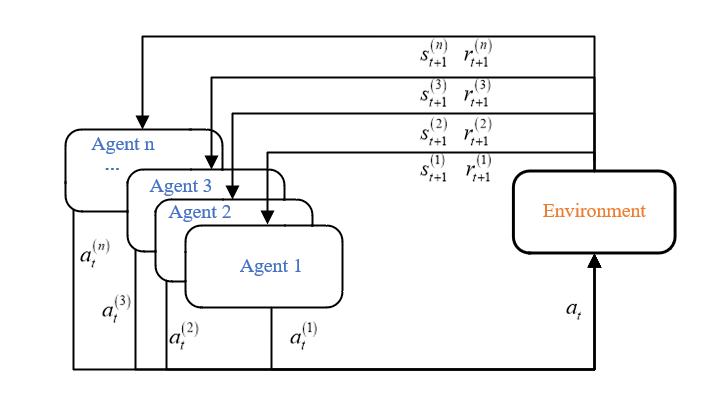
\includegraphics[scale=0.66]{images/multi_agent.png}
    \caption{Progression of a multi-agent reinforcement learning problem}
    \label{fig:multi_agent}
\end{figure*}


\subsection{Experiment Setting}
\label{sec:experiment}

We plan to carry out three major case studies with the simulation environment BlueSky to demonstrate the effectiveness of the D2MARL method. In the three case study listed below, the construction of the virtual sector, intersections,routes and aircraft are all the same. What we change and focus on is the action space.

\subsubsection{Basic Experiment: Action Space With Speed Change Only}

We try to extract the most important behaviors of the aircraft in collision avoidance, we first define the action space mainly based on the changes of the speed:

$$
A_t = \{a_-, 0, a_+\}
$$

Here $A_t$ describes the action an aircraft can take at time $t$. Then $a_-$ is to decrease the speed while $a_+$ is to increase the speed. We use $0$ to represent the action to hold the speed as the corresponding acceraltion equals zero. This means that they should reach the corresponding speed at the next time stamp, which is $v_{t+1}=\{v_{min},v_{t},v_{max}\}$. The speed we use here follow relevant regulations: $v_{min}$ is the minimum allowed cruise speed, $v_{t}$ is the current speed of the aircraft, and $v_{max}$ is the maximum allowed cruise speed. Note that the flight time is divided into several periods, and we allow $\Delta t$ for the plane to take reaction and reach the target speed.

\subsubsection{Route Relaxation: Introduce Direction Change to Actions}

Here we try to make relaxation for an aircraft's route and no longer require the plane to fly along the airlines. We allow the plane to change its flying direction as long as it remain itself inside the airway. This will bring much complexity as the track of the aircraft is on a band rather than along a line. We will allow the aircraft to choose one in three directions:

$$
A_t = \{-\pi / 12, 0, \pi / 12\}
$$

This means that within a time stamp $\Delta t$, the aircraft should be able to turn left or right for 15 degrees.

\subsubsection{Velocity Changes: Combination of Speed and Direction}

In this experiment we will introduce a more complicated action space, that is to allow the aircraft to "truly change its velocity". Considering the fact that in collision avoidance, a plane could have more flexibitity to change its velocity, and that velocity is rather a vector than a scalar, this experiment will be closer to the reality. Combined the first and the second experiment, the action space can be discretized into $3 \times 3 = 9$ actions.



\section{Experiment Result}

In this paragragh we will try to explain how we're going to evaluate our work. We plan to evalute our reinforcement learning model in different aspects, including converge rate, suceess rate and reaction time.

Because the model is designed for a preset sector with specific routes and aircraft and the model could be reused in later operations, the time of training is not the most important thing we consider, but we still hope that the algorithm could converge as soon as possible. As is mentioned above, the air traffic control process is fatal and latency-sensitive, so the success rate and the reaction time are both worth careful consideration.

We propose to record the number of aircraft that leave the sector without collision in the training process and the test process, while the time that agents take each reaction will only be recorded in the test process to ensure that the model is fixed and unchanged.

With such data, we could draw the line chart to show how the success rate raise during the trainging process, and the box-plot to show how our model perform during the test process. The mean and median of the interpretation time could be calculated to show how fast the model react once it's asked to give decision advisories.

\begin{figure}[!htbp]
    \centering
    \subfigure[\label{fig:10aircraft}Episodes vs. Pass Through]{
        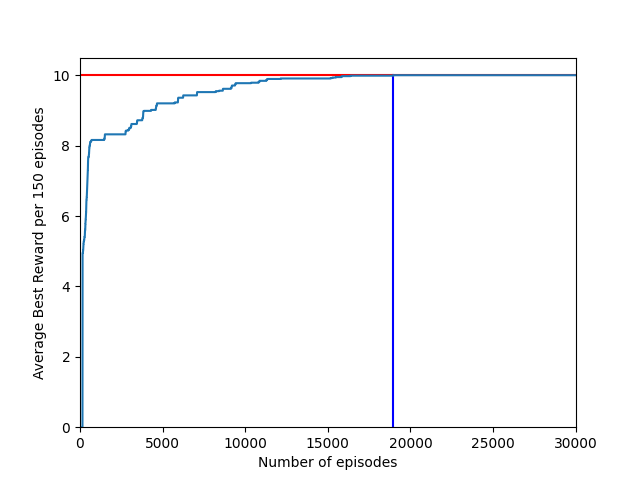
\includegraphics[width=0.3\columnwidth]{images/10aircraft.png}
    }
    \subfigure[\label{fig:30vs50}Influence of Aircrafts]{
        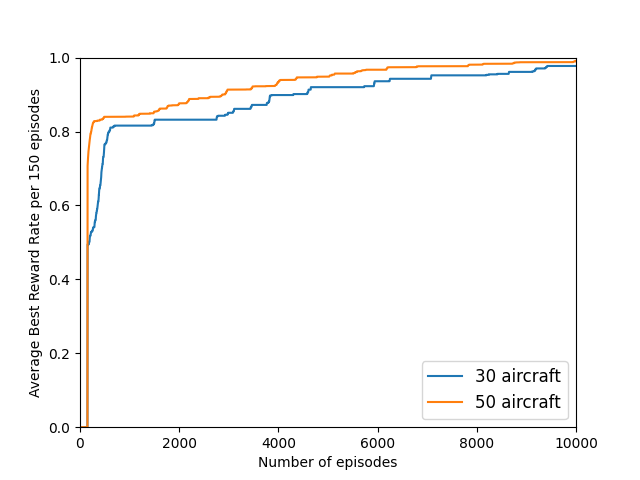
\includegraphics[width=0.3\columnwidth]{images/30vs50.png}
    }
    \subfigure[\label{fig:intruders}Influence of Intruders]{
        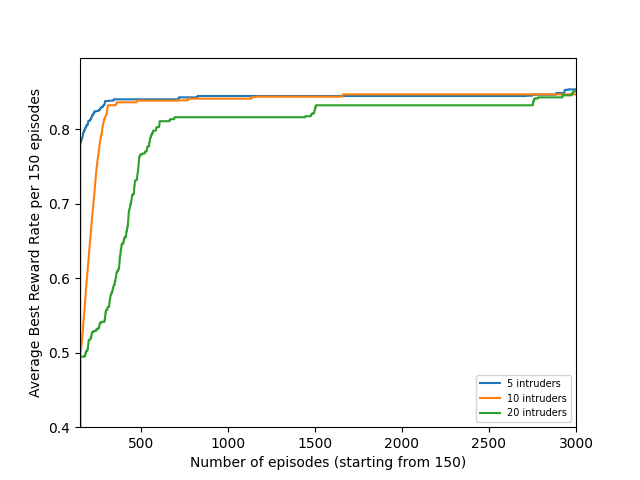
\includegraphics[width=0.3\columnwidth]{images/intruder_influence.png}
    }
    \caption{Experimental Results}
    \label{fig:exp_result}
\end{figure}

From Figure \ref{fig:10aircraft} we can see that the model is actually trainable under our settings. Note that we didn't plot the reward we get every episode since it can vibrates a lot and will cause trouble for us to see the trend. Also the smallest diffence between the reward each time is 2 rather than 1 since we defined the reward as the number of aircraft that leave the sector successfully. Instead, we record the average reward every 150 episodes.

We also try to check whether using information from some of rather than all of other planes could be effective. We fix the n-sate as 5, so the sample rate could change from 50\% to 16.7\% when we change the maximum number of aircrafts in the sector from 30 to 50. From Figure \ref{fig:30vs50} we can see that the convergence result didn't get worse.

The number of intruders could also influence the converge speed. Checking the \textit{150-th} to the \textit{3000-th} episodes, we can see such result. The reason might be more intruders potentially increase the difficulty to pass through. However, this will not influence the process of convergence. The result is shown on Figure \ref{fig:intruders}.
%\input{sections/result_analysis.tex}
\section{Conclusion}
A deep multi-agent reinforcement learning framework is proposed in this paper to tackle mid-air collision avoidance problems in a structured sector with multiple intersections and emerging points. We have formualted our case studies by allowing aircraft to change the both the desired speed and direction. The results implemented by the D2MARL formeworl shows that nearly all aircraft avoidance can be solved. It also shows that the results can provide a novel idea to the development of future autonomous air traffic control system.

To some extent, our experimental results show that our proposed D2MARL can solve the mid-air collision avoidance problem in our defined framework. But there still exsit some improvements when considering more complex and practical scenarios, such as 4-D aircraft trajectories conflict detection and resolution. Besides, we plan to further employ an attention mechanism and encourage cooperation beyond communication among the agents in our proposed framework, to obtain more satisfying results and learning efficency.


\input{sections/algorithm.tex}

\bibliographystyle{unsrtnat}
\bibliography{references}  %%% Uncomment this line and comment out the ``thebibliography'' section below to use the external .bib file (using bibtex) .


%%% Uncomment this section and comment out the \bibliography{references} line above to use inline references.
% \begin{thebibliography}{1}

% 	\bibitem{kour2014real}
% 	George Kour and Raid Saabne.
% 	\newblock Real-time segmentation of on-line handwritten arabic script.
% 	\newblock In {\em Frontiers in Handwriting Recognition (ICFHR), 2014 14th
% 			International Conference on}, pages 417--422. IEEE, 2014.

% 	\bibitem{kour2014fast}
% 	George Kour and Raid Saabne.
% 	\newblock Fast classification of handwritten on-line arabic characters.
% 	\newblock In {\em Soft Computing and Pattern Recognition (SoCPaR), 2014 6th
% 			International Conference of}, pages 312--318. IEEE, 2014.

% 	\bibitem{hadash2018estimate}
% 	Guy Hadash, Einat Kermany, Boaz Carmeli, Ofer Lavi, George Kour, and Alon
% 	Jacovi.
% 	\newblock Estimate and replace: A novel approach to integrating deep neural
% 	networks with existing applications.
% 	\newblock {\em arXiv preprint arXiv:1804.09028}, 2018.

% \end{thebibliography}

\appendix

% \section{Project Progress Structure Explanation}

% The relationship between the outline and our report is shown on figure \ref{fig:mapping}. Here we note that the scenario and goals are not fully intruduced in only one paragragh, while the details of our implementation plan and schedule could be viewed from the table attached in the appendix. The implementation plan might change during the process of our work, judging from our actual progress.

% \begin{figure*}[htbp]
% \centering
% 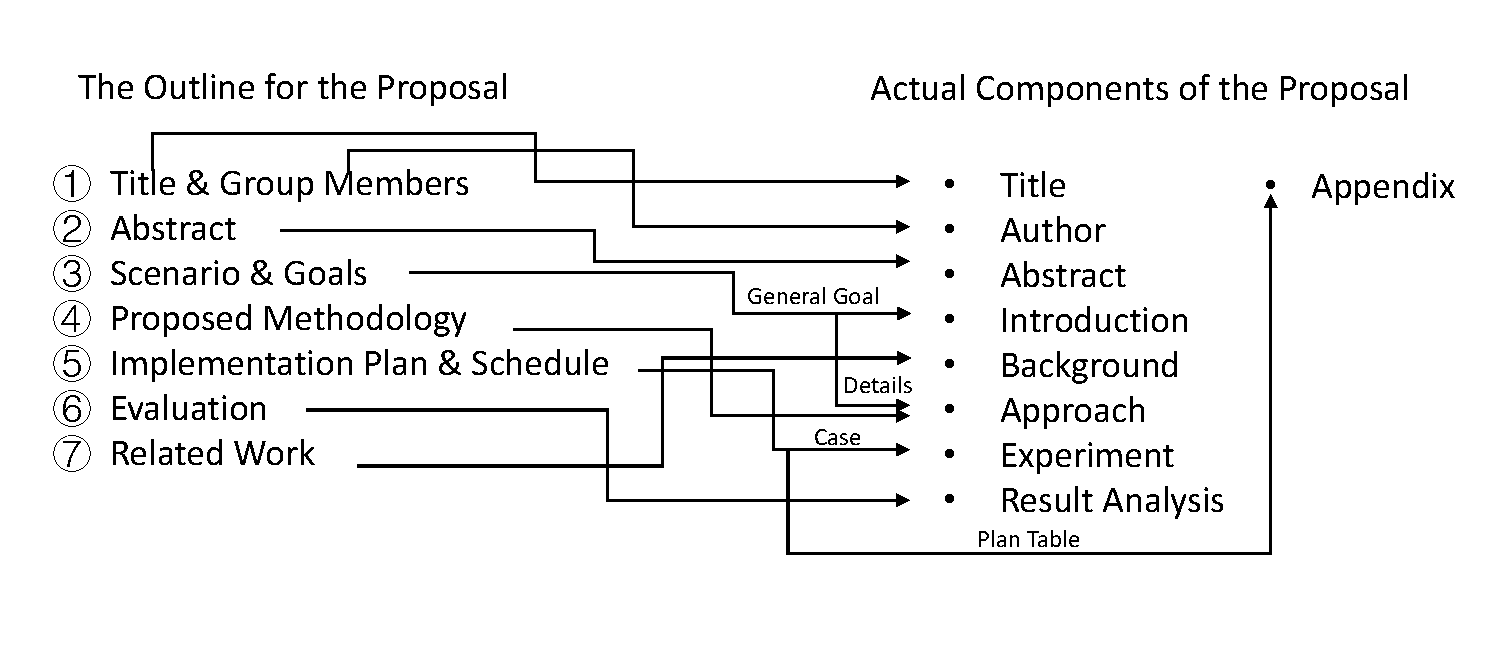
\includegraphics[scale=0.45]{images/mapping.pdf}
% \caption{The relationship between the outline of the proposal and the actual proposal structure}
% \label{fig:mapping}
% \end{figure*}

\section{Schedule and Contribution}
Our project progression and specific assignment arrangement is showed as Table 1. For the project report, Weilin Cai is mainly responsible for introduction, modeling, experiment setting, experiment result while Chi Li is mainly responsible for background, modeling, algorithm and conclusion.
\begin{table}[htbp]
	\caption{Implementation Plan and Schedule}
	\centering
	\begin{tabular}{|p{.1\linewidth} < {\centering}| p{.4\linewidth} < {\centering} | p{.4\linewidth} < {\centering} |}
	\hline
			   & \textbf{Weilin Cai} & \textbf{Chi Li} \\ \hline
		Week 1 & Study the usage of Tensorflow \& BlueSky & Gather domain knowledge \\ \hline
		Week 2 & \multicolumn{2}{c|}{Accomplish D2MARL modeling via Reinforcement Learning}													\\ \hline
		Week 3 & \multicolumn{2}{c|}{Start the basic experiment where the action can be speed-changes only}                                                                                  \\ \hline
		Week 4 & Organize and summarize experimental results & Finish the midterm project progress report                                 \\ \hline
		Week 5 & \multicolumn{2}{c|}{Action space with direction change}                                                                                        \\ \hline
		Week 6 &  Action space with velocity                                    &  State Feature Extraction                                 \\ \hline
		Week 7 & PPO convergence rate test  & Analyze the Convergence Result                                                    \\ \hline
		Week 8 & \multicolumn{2}{c|}{Finish the final research report and poster}    \\ \hline              
 \end{tabular}

\end{table}

\section{The Repostitory of This Project}

We put the resoures of our project on \emph{Github}. You can visit \href{https://github.com/WhiskyChoy/rl-project.git}{https://github.com/WhiskyChoy/rl-project.git} to check our project. Files like the proposal and the midterm report are inside the \verb|Documents| directory. Source codes are stored in the \verb|Codes| directory and you can run the program following the instruction of the \verb|readme.md| file.

\end{document}